% JUMP TO LINE 60, 75
\documentclass[preview, margin=0.6in]{standalone}
\usepackage[letterpaper,portrait,top=0.4in, left=0.6in, right=0.6in, bottom=1in]{geometry}

\usepackage{amsmath, amsfonts, amsthm, amssymb}
\usepackage{graphicx, float}
\usepackage{mathtools}
\usepackage{titlesec}
\usepackage{interval}
\usepackage{hyperref}
\usepackage{siunitx}
\usepackage{titling}
\usepackage{vwcol}
\usepackage{setspace}
\usepackage{empheq}
\usepackage{cancel}
\usepackage{esdiff}
\usepackage{multicol}
\usepackage{mdframed}
\usepackage{esdiff}
\usepackage{tikzsymbols}
\usepackage{multicol}
\usepackage{tikz}
\usepackage{varwidth}
\usepackage{parskip}
\usepackage{pgfplots}
\pgfplotsset{compat=1.18}
\intervalconfig {
	soft open fences
}

\newcommand{\alignedintertext}[1]{%
  \noalign{%
    \vskip\belowdisplayshortskip
    \vtop{\hsize=\linewidth#1\par
    \expandafter}%
    \expandafter\prevdepth\the\prevdepth
  }%
}

\newtheorem{lemma}{Lemma}

\renewcommand{\qedsymbol}{\Smiley[1.3]}
\newcommand*{\problem}[1]{\section*{Problem #1}}
\newcommand*{\aps}{\section*{AP Corner}}
\newcommand*{\deriv}[1][x]{\ensuremath{\dfrac{\mathrm{d}}{\mathrm{d}#1}}}
\newcommand*{\floor}[1]{\ensuremath{\lfloor #1\rfloor}}
\newcommand*{\lheqzero}{\ensuremath{\underset{\text{L'H}}{\overset{\left[\frac00\right]}{=}}}}
\newcommand*{\lheqinfty}{\ensuremath{\underset{\text{L'H}}{\overset{\left[\frac{\infty}{\infty}\right]}{=}}}}

\DeclareMathOperator{\DNE}{DNE}
\DeclareMathOperator{\sgn}{sgn}

\DeclareMathOperator{\arccsc}{arccsc}
\DeclareMathOperator{\arcsec}{arcsec}
\DeclareMathOperator{\arccot}{arccot}

%opening

\title{\vspace*{-30pt}Problem Set \#40}
\author{Jayden Li}
\date{\today}

% \allowdisplaybreaks
\postdisplaypenalty=100000

\begin{document}
\setstretch{1.25}
\fontsize{12pt}{12pt}\selectfont
\setlength{\abovedisplayskip}{0pt}
\setlength{\parindent}{0pt}
\setlength{\parskip}{2ex plus 0.5ex minus 0.2ex}
\maketitle

\problem{5}
Let $a_n$ be the amount of money received by the $n$th person. $a_n=Dc^{n-1}$.
\begin{itemize}
	\item[(a)]
		$\displaystyle S_n=\sum_{k=1}^{n}S_k=\sum_{k=1}^{n}Dc^{k-1}$

	\item[(b)]
		$\begin{aligned}[t]
			\lim_{n\to\infty}S_n
			=D\sum_{i=1}^{\infty}c^{i-1}
			=\frac{D}{1-c}
			=\frac{D}{s}
			=\underbrace{\frac{1}{s}}_{k}D
		\end{aligned}$

		$\text{Marginal propensity to consume}=c=0.8$ then $\text{multiplier}=k=1/s=1/(1-c)=1/0.2=5$.

\end{itemize}

\problem{8}
\begin{itemize}
	\item[(a)]
		\phantom{}

		\begin{center}
			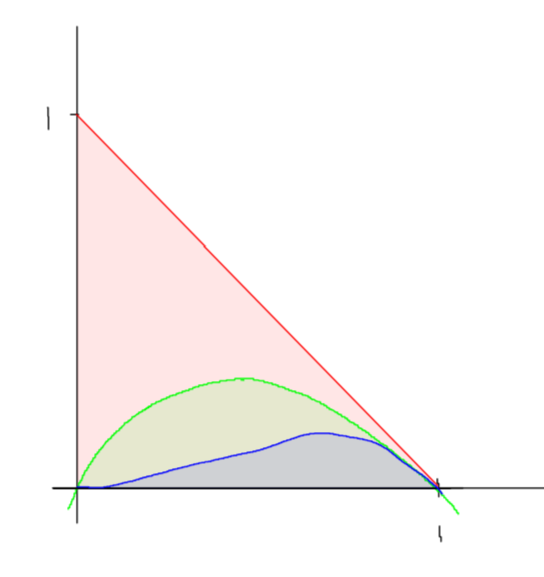
\includegraphics[width=0.5\linewidth]{q8a.png}
		\end{center}

	\item[(b)]
		\begin{align*}
		    \int_{0}^{1}(1-x)\,\mathrm{d}x
			&=\left[x-\frac{x^2}{2}\right]_{0}^{1}
			=1-\frac{1}{2}
			=\frac{1}{2} \\
			\int_{0}^{1}\left(x-x^2\right)\mathrm{d}x
			&=\left[\frac{x^2}{2}-\frac{x^3}{3}\right]_{0}^{1}
			=\frac12-\frac13
			=\frac16 \\
			\int_{0}^{1}\left(x^2-x^3\right)\mathrm{d}x
			&=\left[\frac{x^3}{3}-\frac{x^4}{4}\right]_{0}^{1}
			=\frac13-\frac14
			=\frac1{12}
		\end{align*}

	\item[(c)]
		$\begin{aligned}[t]
			a_n
			&=\int_{0}^{1}\left(x^{n-1}-x^n\right)\mathrm{d}x
			=\left[\frac{x^n}{n}-\frac{x^{n+1}}{n+1}\right]_{0}^{1}
			=\frac{1}{n}-\frac{1}{n+1}
			=\frac{n+1-n}{n(n+1)}
			=\boxed{\frac{1}{n^2+n}} \\
			\sum_{n=1}^{\infty}a_n
			&=\sum_{n=1}^{\infty}\int_{0}^{1}\left(x^{n-1}-x^n\right)\mathrm{d}x
			=\int_{0}^{1}\left(x^0-\cancel{x^1}+\cancel{x^1}-\cancel{x^2}+\ldots+\cancel{x^{n-1}}-x^n\right)\mathrm{d}x
			=\int_{0}^{1}\left(1-x^n\right)\mathrm{d}x \\
			&=\left[x-\frac{x^{n+1}}{n+1}\right]_{0}^{1}
			=1-\frac{1}{n+1}
			=\frac{n+1}{n+1}-\frac{1}{n+1}
			=\boxed{\frac{n}{n+1}}
		\end{aligned}$

\end{itemize}
\end{document}
